Le prétraitement de ces données est divisé en deux étapes principales. La première concerne des aspects plus simples : l'élimination des données nulles et la vérification de la longueur des textes en excluant les valeurs aberrantes. La deuxième concerne le sens de ces textes, afin de vérifier l'homogénéité de leur contenu. Aux fins du présent article, il convient de se concentrer uniquement sur la deuxième phase.
\\

L'objectif final est de vérifier que les textes du dataset, bien que provenant de sources différentes, ont des significations similaires. Pour ce faire, nous avons d'abord transformé les phrases en un vecteur numérique - ce que l'on appelle "embedding" dans le domaine du traitement automatique des langues. Cette transformation a été effectuée à l'aide d'un modèle de sentence embeddings dérivé du modèle de langue BERT. L'architecture de sentence-BERT et ses détails techniques sont présentés dans \underline{\href{https://arxiv.org/abs/1908.10084}{cet article}}\footcite{reimers2019}.  \\
En particulier, le modèle utilisé est \emph{sentence-bert-base-italian-xxl-uncased}\footcite{sentenceBERT2024}, qui est dérivé du modèle \emph{bert-base-italian-xxl-uncased}. Il s'agit d'un modèle BERT entraîné sur des données italiennes provenant des corpus OPUS et OSCAR. \\

Pour entrer dans les détails techniques, les embeddings ont été obtenus à l'aide de la librairie python Sentence Transformer. Les résultats ont ensuite été enregistrés dans une matrice numpy de la forme (95442, 768). À ce stade, les techniques de réduction dimensionnelle suivantes ont été utilisées pour visualiser ces données : analyse en composantes principales (PCA) et UMAP. La visualisation de ces données à travers ces technique nous permet de voir s'il existe des \emph{cluster} particuliers en fonction de la source des données. Les représentations graphiques des réductions dimensionnelles sont présentées ci-dessous. La couleur des points dépend de la source des données.

\begin{figure}[h!]
	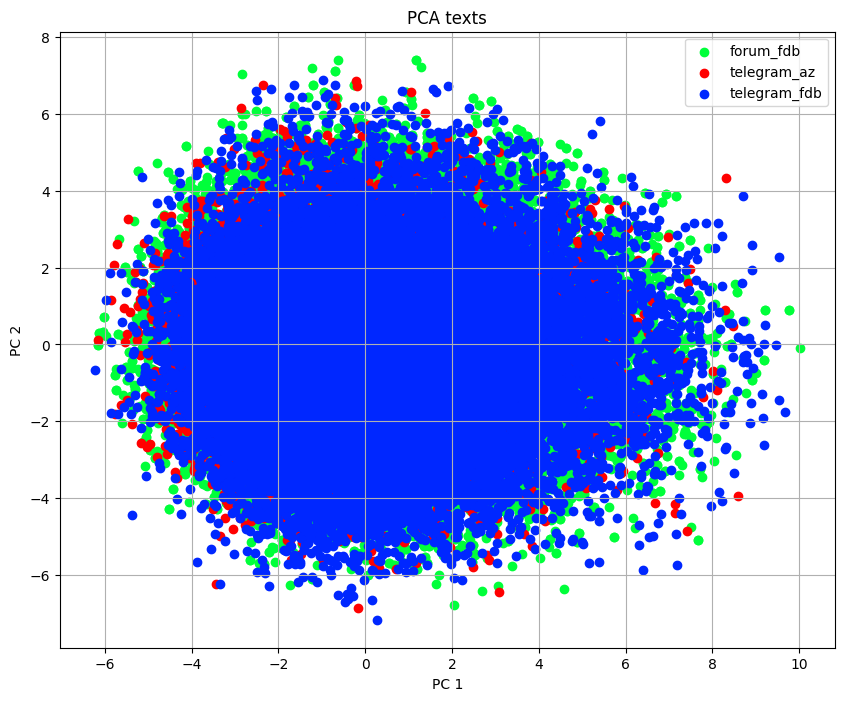
\includegraphics[scale=0.5]{PCA.png}
	\centering
	\caption{Plot des données réduites par PCA}
\end{figure}

\begin{figure}[h!]
	\includegraphics[scale=0.5]{umap.png}
	\centering
	\caption{Plot des données réduites par UMAP}
\end{figure}

\clearpage

Comme on peut le voir, les graphiques ressemblent à une multitude de points sans \emph{pattern} particuliers. Tant dans le cas de la PCA que dans celui de l'UMAP, il n'y a pas de cluster en fonction de la couleur. Cela montre que les textes ont une signification homogène quelle que soit leur source.